%=========================================================
% Capítulo 4 — Ajustes em duas dimensões e função de suavização
%=========================================================
\chapter{Ajustes em duas dimensões e função de suavização}
\label{ch:ajustes2d}

\noindent\textbf{Resumo:}
Neste capítulo, generalizamos o método dos mínimos quadrados para duas dimensões e introduzimos o conceito de \emph{suavização}.  
Mostra-se como o controle da variabilidade espacial conduz naturalmente aos métodos de análise objetiva usados em meteorologia e assimilação de dados.  
A ideia central é encontrar o equilíbrio entre fidelidade aos dados e coerência espacial do campo analisado.

%---------------------------------------------------------
\section{Extensão para duas dimensões}
Até agora tratamos de variáveis unidimensionais.  
Em meteorologia, porém, buscamos reconstruir campos como temperatura, pressão ou vento sobre uma área bidimensional.  
Dado um conjunto de observações $\{(x_i, y_i, z_i)\}_{i=1}^{N}$, queremos estimar uma função contínua $f(x,y)$ que represente o campo.  
Podemos expressá-la em uma base bidimensional:
\begin{equation}
f(x,y) = \sum_{j=1}^{M} a_j \, \phi_j(x,y),
\label{eq:basis2d}
\end{equation}
onde $\phi_j$ são funções de base (por exemplo, polinômios em $x$ e $y$ ou funções radiais).  
A minimização do erro global
\begin{equation}
J = \sum_{i=1}^{N} \big[z_i - f(x_i,y_i)\big]^2
\label{eq:2d-cost}
\end{equation}
segue a mesma lógica do capítulo anterior, resultando em equações normais análogas.  
A diferença está no tipo de função base escolhida e na necessidade de regularizar o ajuste.

%---------------------------------------------------------
\section{A necessidade de suavização}
Quando o número de pontos é grande ou o campo contém ruído, ajustes exatos produzem oscilações não físicas (Figura~\ref{fig:2d-raw}).  
Introduzimos então um termo de \emph{suavização} na função custo:
\begin{equation}
J_s = \sum_{i=1}^{N} \big[z_i - f(x_i,y_i)\big]^2
+ \lambda \iint \left[ \left(\frac{\partial^2 f}{\partial x^2}\right)^2
+ \left(\frac{\partial^2 f}{\partial y^2}\right)^2 \right] dx\,dy.
\label{eq:smooth-cost}
\end{equation}
O parâmetro $\lambda$ controla o compromisso entre fidelidade e suavidade:
\begin{itemize}
  \item $\lambda \to 0$: ajuste quase exato (pode oscilar);
  \item $\lambda \to \infty$: campo excessivamente suave (subestima variações reais).
\end{itemize}
Essa regularização dá origem às técnicas de \emph{análise objetiva}, como as de Cressman e Barnes, nas quais o campo é filtrado por uma função de ponderação espacial.

%---------------------------------------------------------
\section{Interpretação física e estatística}
Em termos físicos, o termo de suavização impõe coerência espacial, equivalente a exigir que o campo tenha continuidade e derivadas limitadas — algo análogo à difusão.  
Em termos estatísticos, a regularização equivale a assumir correlações espaciais finitas entre os erros.  
Na assimilação de dados, essa correlação é descrita pela matriz de covariância $B$, cuja estrutura (gaussiana, exponencial, etc.) define a “suavidade” da análise.

%---------------------------------------------------------
\section{Funções de ponderação e filtros espaciais}
A interpolação bidimensional pode ser escrita como:
\begin{equation}
\hat{f}(x,y) = \frac{\displaystyle \sum_{i=1}^{N} W_i(x,y)\, z_i}
                     {\displaystyle \sum_{i=1}^{N} W_i(x,y)},
\label{eq:weighted2d}
\end{equation}
em que $W_i(x,y)$ são funções de peso que decaem com a distância:
\[
W_i(x,y) = \exp\!\left[-\frac{(x-x_i)^2 + (y-y_i)^2}{R^2}\right],
\]
com $R$ sendo o raio de influência.  
Essa forma é o ponto de partida para o método de Barnes e outros esquemas de análise objetiva, em que $R$ e $\lambda$ são ajustados para balancear ruído e detalhe.

%---------------------------------------------------------
\section{Exemplo visual em 2D (pgfplots)}
As Figuras~\ref{fig:2d-raw} e \ref{fig:2d-smooth} ilustram o efeito da suavização sobre um campo de pontos amostrados aleatoriamente.

\begin{figure}[h!]
\centering
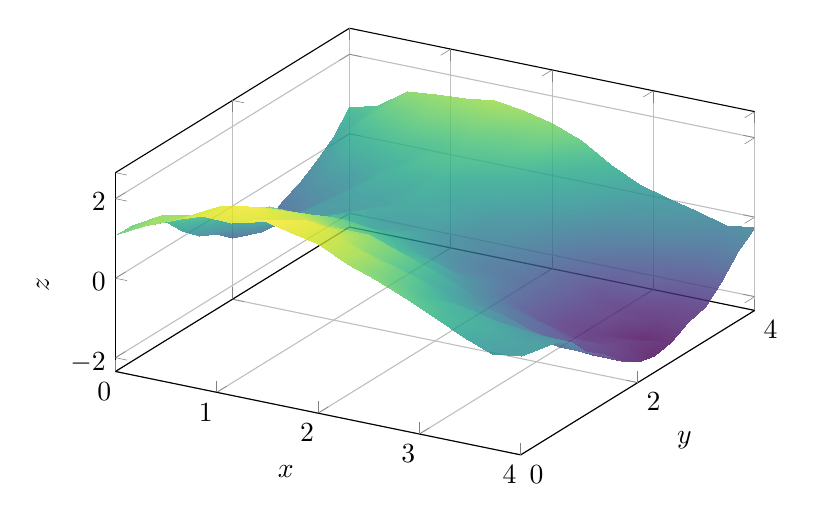
\begin{tikzpicture}
  \begin{axis}[
    view={30}{40},
    width=0.8\linewidth, height=7cm,
    xlabel={$x$}, ylabel={$y$}, zlabel={$z$},
    domain=0:4, y domain=0:4,
    grid=both, samples=15,
    colormap/viridis,
  ]
    \addplot3[surf, opacity=0.8, shader=interp]
      {sin(deg(x*1.2)) + cos(deg(y*1.3)) + 0.3*rnd};
  \end{axis}
\end{tikzpicture}
\caption{Campo interpolado diretamente (sem suavização): as flutuações aleatórias geram ruído visível.}
\label{fig:2d-raw}
\end{figure}

\begin{figure}[h!]
\centering
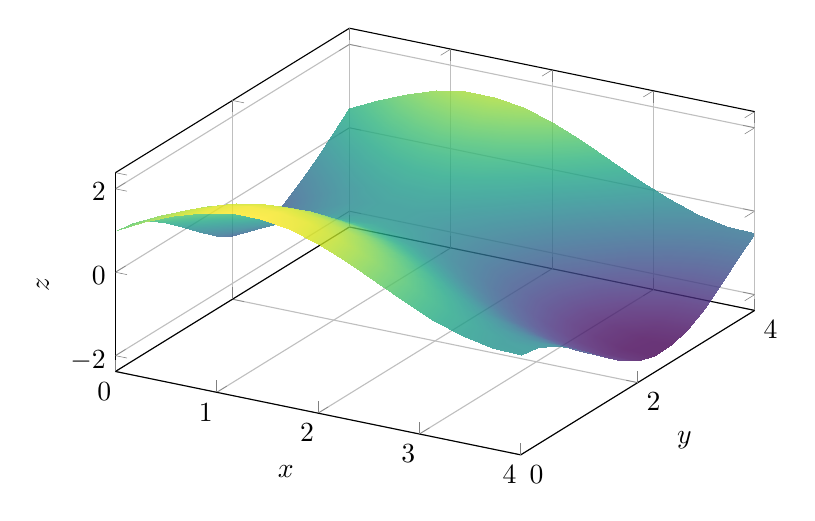
\begin{tikzpicture}
  \begin{axis}[
    view={30}{40},
    width=0.8\linewidth, height=7cm,
    xlabel={$x$}, ylabel={$y$}, zlabel={$z$},
    domain=0:4, y domain=0:4,
    grid=both, samples=15,
    colormap/viridis,
  ]
    \addplot3[surf, opacity=0.8, shader=interp]
      {sin(deg(x*1.2)) + cos(deg(y*1.3))};
  \end{axis}
\end{tikzpicture}
\caption{Campo suavizado com regularização: o ruído é atenuado, preservando as estruturas principais.}
\label{fig:2d-smooth}
\end{figure}

%---------------------------------------------------------
\section{Conexão com análise objetiva}
A adição do termo de suavização em \eqref{eq:smooth-cost} e o uso de pesos espaciais em \eqref{eq:weighted2d} constituem a base da \emph{análise objetiva} (\emph{Objective Analysis} ou OBAN).  
Essas ideias foram aplicadas na meteorologia operacional antes da era dos supercomputadores e ainda hoje fundamentam métodos como Cressman (1959) e Barnes (1964).  
A diferença é que, na assimilação moderna, a suavização e os pesos são determinados de forma \emph{ótima} a partir das estatísticas de erro — um avanço direto do que começou aqui.

%---------------------------------------------------------
\section{Síntese}
A generalização para duas dimensões e a introdução da suavização marcaram a transição da interpolação geométrica para a análise estatística.  
Os parâmetros de suavidade e raio de influência representam fisicamente a correlação espacial dos erros e matematicamente o filtro aplicado ao campo analisado.  
No próximo capítulo, exploraremos como esses conceitos foram formalizados nos métodos clássicos de análise objetiva — a ponte definitiva entre interpolação e assimilação de dados.

% Fim do Capítulo 4
